\chapter{Methodology and Schedule} 
\epigraph{There is no greater harm than that of time wasted.}{Michelangelo}

\section{Methodology}
Tools for characterizing and analyzing performance on each specific scenario will be identified and integrated on the testing platforms. There are existing open source tools that provide the required information, but little information regarding specific use to instrument the desired scenarios.

The following are the specific scenarios that will be evaluated on each platform:
\begin{itemize*}
\item Video capture, and encoding.
\item Audio capture, and encoding.
\item Synchronized video and audio capture, encoding and storage in block-based storage devices using an standard multimedia file container.
\item Synchronized video and audio capture, encoding and transmission over network using RTP/UDP/IP protocol.
\item Video decoding and preview from block-based storage devices using a standard multimedia file container.
\end{itemize*}

For block-based storage devices, we consider any storage device with semantics similar to that of standard hard disks, and specifically excluding devices based on flash memory unless they use any sort of \ac{FTL}.

The following aspects will be considered for each specific scenario:
\begin{itemize*}
\item CPU usage and scheduling overhead.
\item Memory usage and overhead by the software stack.
\item I/O usage: efficiency regarding use of the specific I/O architecture and overhead by the software stack.
\end{itemize*}

\section{List of Deliveries}
The deliveries are:
\begin{enumerate*}
\item Patches for the Linux kernel available for the specific platforms to improve their performance.
\item Patches for GStreamer to improve performance on the target scenarios and platforms.
\end{enumerate*}

As stated previously, all the patches will be designed with the intention of being accepted into their respective projects, but no guarantee is made about their merging on mainstream. Still, the work will be done while interacting with the respective project maintainers.

\newpage
\section{Schedule and Work Breakdown}

\begin{table}[tph]
\caption{Work Breakdown} \centering
\begin{tabular}{c}
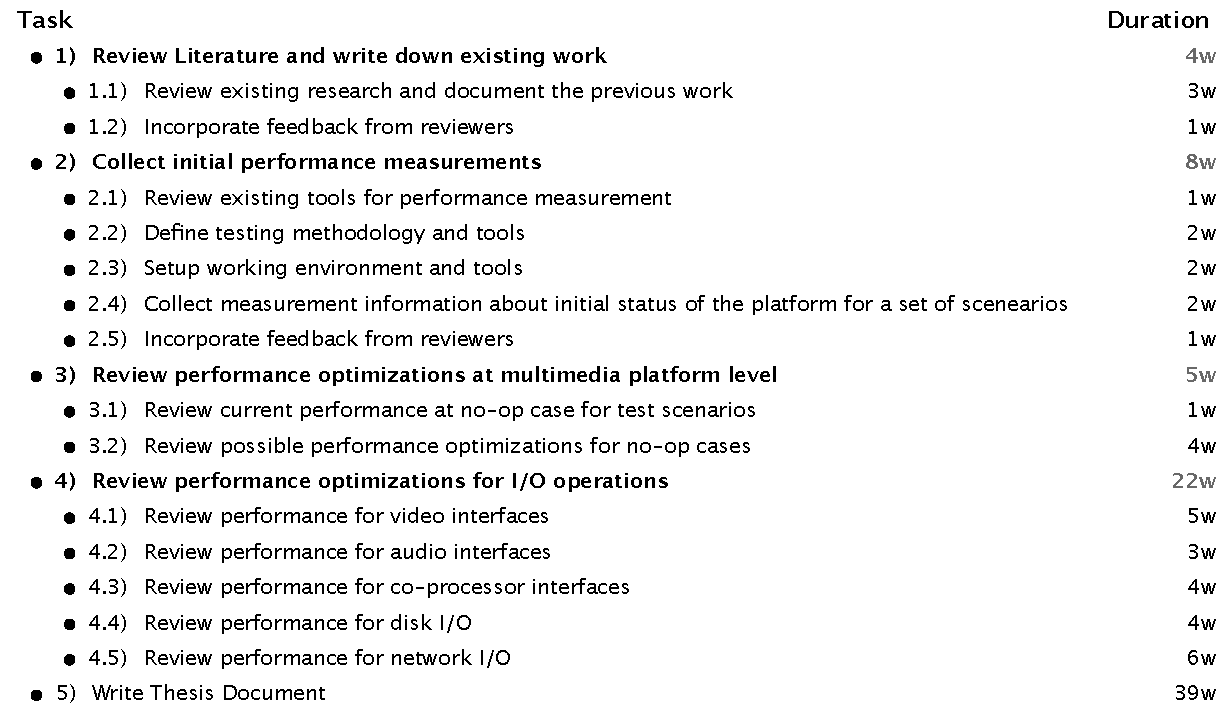
\includegraphics[width=1.0\textwidth]{images/Outline.pdf}
\end{tabular}
\end{table}

\begin{figure}[tbh]
\centering
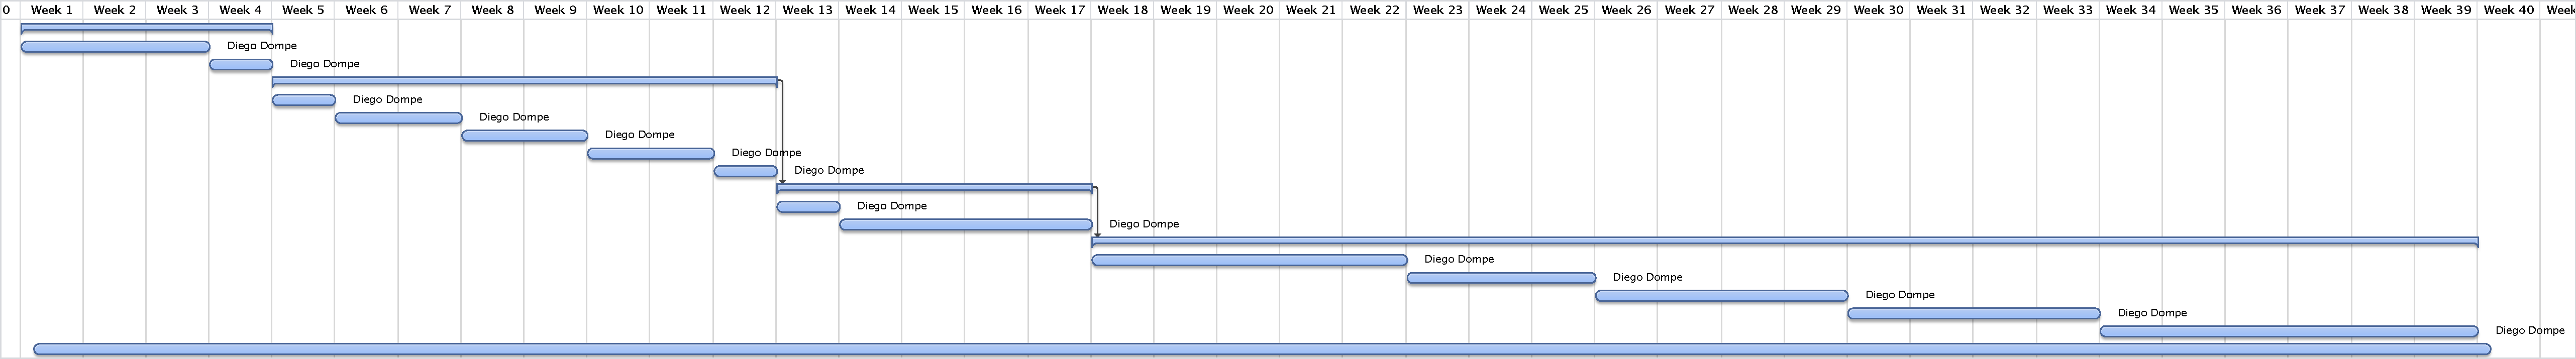
\includegraphics[width=0.55\textheight,height=0.34\textwidth,angle=90]{images/Gantt.pdf}\\
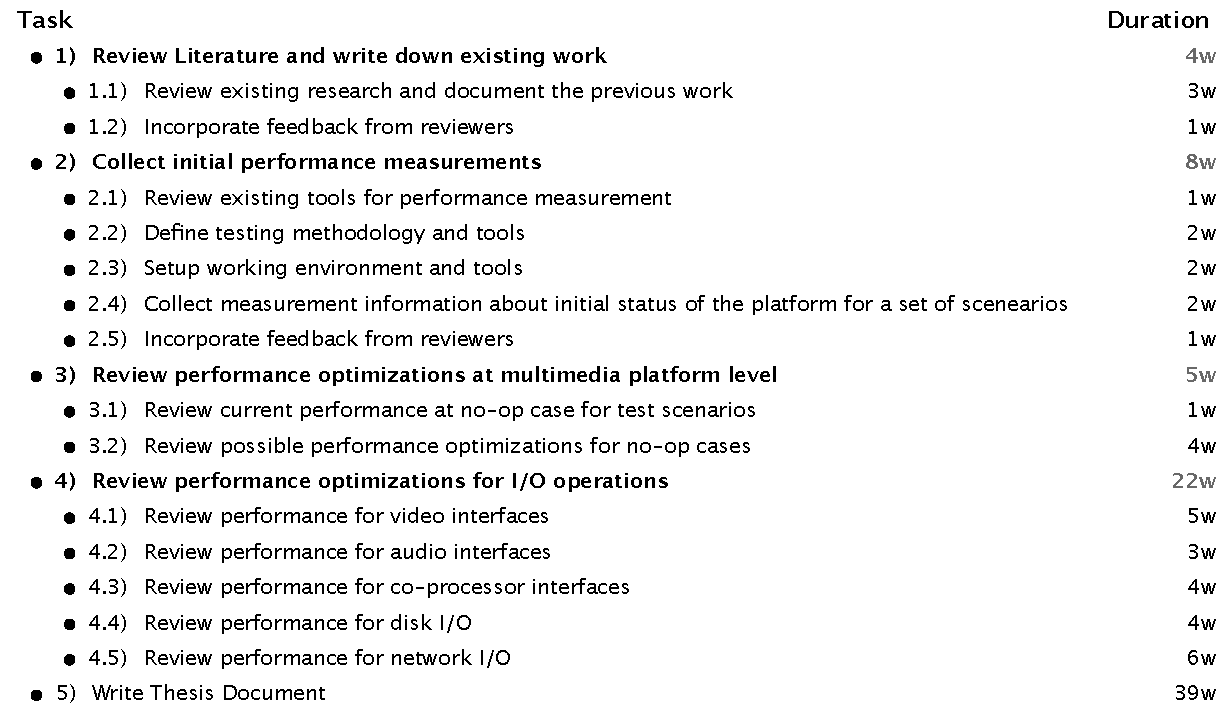
\includegraphics[width=0.4\textheight,angle=90]{images/Outline.pdf}
\caption{Gantt Chart}\label{gantt}
\end{figure}
